% begin module polar-many-representations
\begin{frame}
\begin{columns}[c]
\column{.5\textwidth}
\ \uncover<1->{%
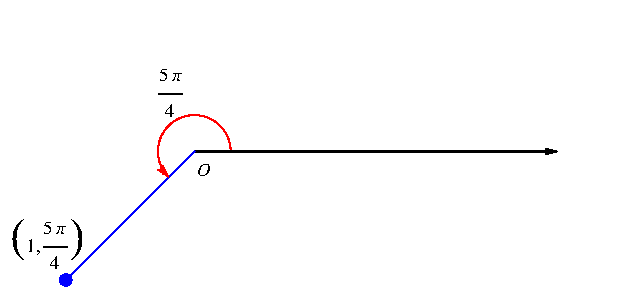
\includegraphics[height=3cm]{polar-curves/pictures/11-03-ex1a.pdf}%
}%

\ \uncover<2->{%
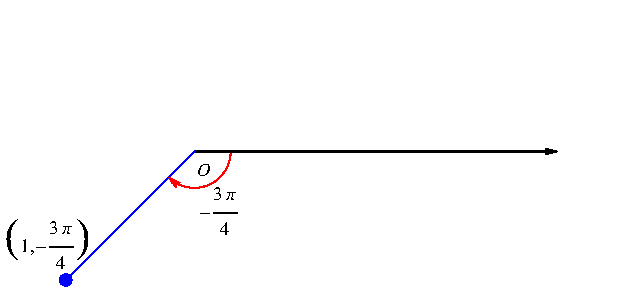
\includegraphics[height=3cm]{polar-curves/pictures/11-03-ex1b.pdf}%
}%
\column{.5\textwidth}
\ \uncover<3->{%
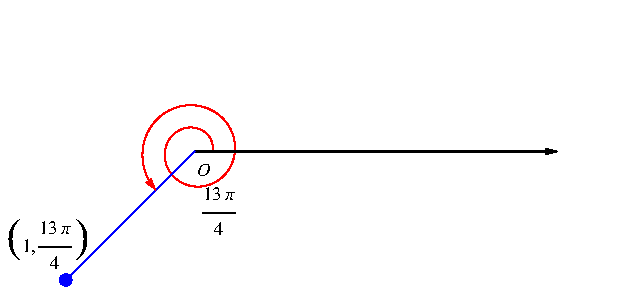
\includegraphics[height=3cm]{polar-curves/pictures/11-03-ex1c.pdf}%
}%

\ \uncover<4->{%
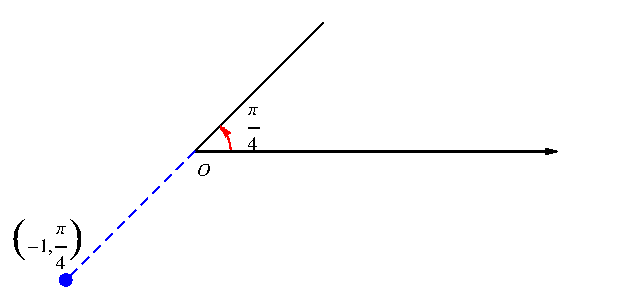
\includegraphics[height=3cm]{polar-curves/pictures/11-03-ex1d.pdf}%
}%
\end{columns}
\begin{itemize}
\item  There are many ways to represent the same point.
\item<2-| alert@2>  We could use a negative $\theta$.
\item<3-| alert@3>  We could go around more than once.
\item<4-| alert@4>  We could use a negative $r$.
\end{itemize}
\end{frame}
% end module polar-many-representations
